\documentclass{standalone}
\usepackage{tikz}
\usetikzlibrary{patterns, positioning}


\begin{document}
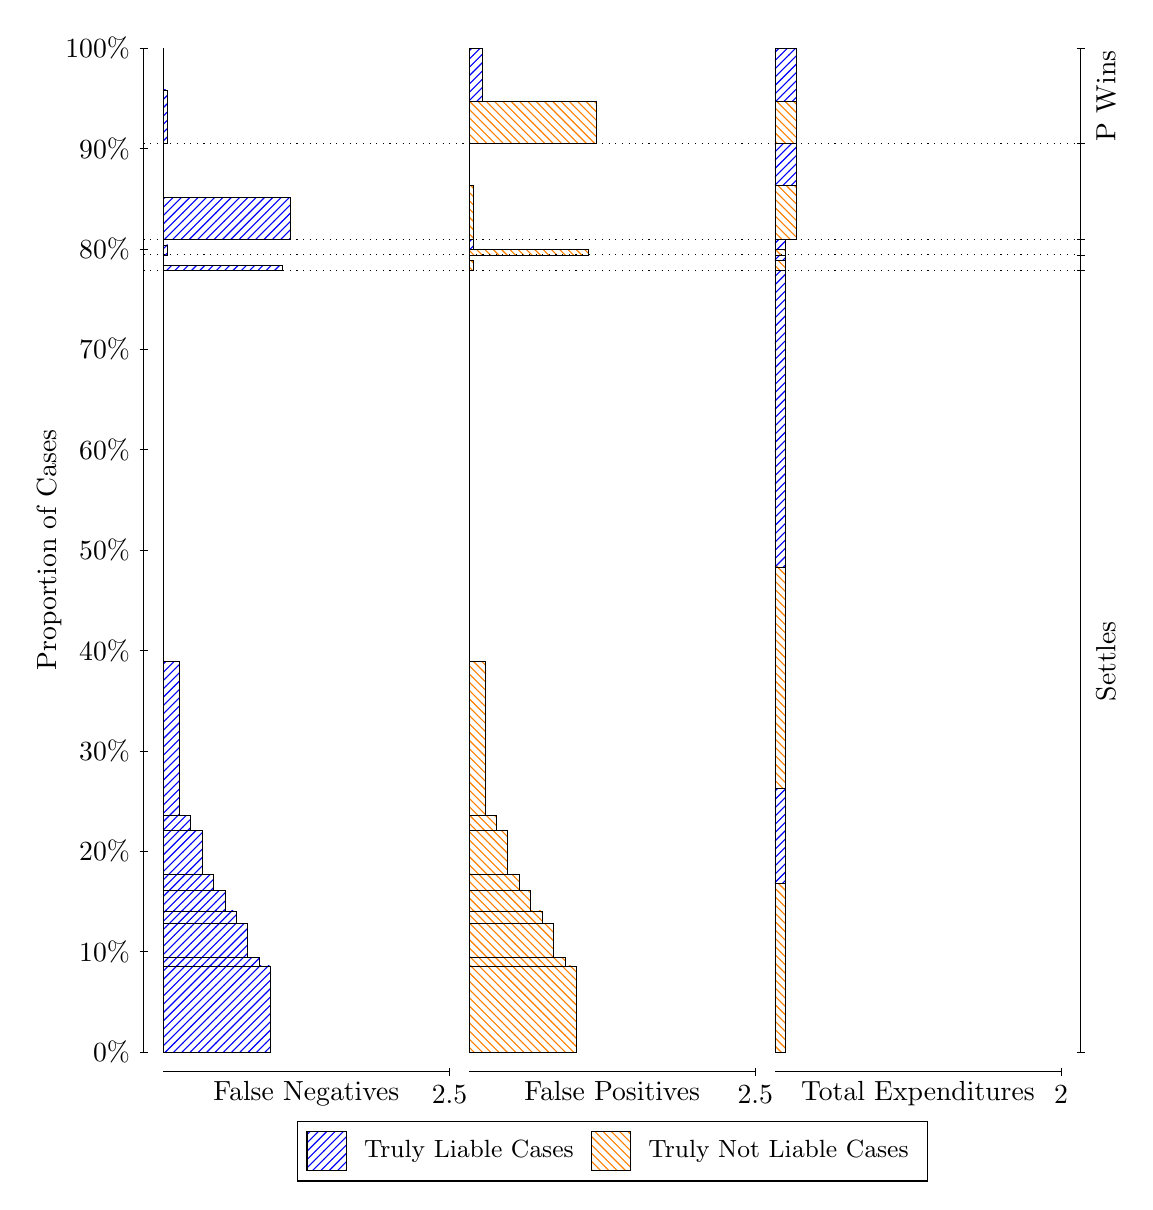
\begin{tikzpicture}
\draw[black, very thin] (1.5,1.75) -- (1.5,14.5);
\node[rotate=90, text=black, anchor=center] at (0.3, 8.125) {Proportion of Cases};
\draw[black, very thin] (1.45,1.75) -- (1.55,1.75);
\node[text=black, anchor=east] at (1.45, 1.75) {0\%};
\draw[black, very thin] (1.45,3.025) -- (1.55,3.025);
\node[text=black, anchor=east] at (1.45, 3.025) {10\%};
\draw[black, very thin] (1.45,4.3) -- (1.55,4.3);
\node[text=black, anchor=east] at (1.45, 4.3) {20\%};
\draw[black, very thin] (1.45,5.575) -- (1.55,5.575);
\node[text=black, anchor=east] at (1.45, 5.575) {30\%};
\draw[black, very thin] (1.45,6.85) -- (1.55,6.85);
\node[text=black, anchor=east] at (1.45, 6.85) {40\%};
\draw[black, very thin] (1.45,8.125) -- (1.55,8.125);
\node[text=black, anchor=east] at (1.45, 8.125) {50\%};
\draw[black, very thin] (1.45,9.4) -- (1.55,9.4);
\node[text=black, anchor=east] at (1.45, 9.4) {60\%};
\draw[black, very thin] (1.45,10.675) -- (1.55,10.675);
\node[text=black, anchor=east] at (1.45, 10.675) {70\%};
\draw[black, very thin] (1.45,11.95) -- (1.55,11.95);
\node[text=black, anchor=east] at (1.45, 11.95) {80\%};
\draw[black, very thin] (1.45,13.225) -- (1.55,13.225);
\node[text=black, anchor=east] at (1.45, 13.225) {90\%};
\draw[black, very thin] (1.45,14.5) -- (1.55,14.5);
\node[text=black, anchor=east] at (1.45, 14.5) {100\%};

\draw[black, very thin] (13.4,1.75) -- (13.4,14.5);
\draw[black, very thin] (13.35,1.75) -- (13.45,1.75);
\node[anchor=west] at (13.35, 1.75) {};
\draw[black, very thin] (13.35,11.675) -- (13.45,11.675);
\node[anchor=west] at (13.35, 11.675) {};
\draw[black, very thin] (13.35,11.873) -- (13.45,11.873);
\node[anchor=west] at (13.35, 11.873) {};
\draw[black, very thin] (13.35,12.071) -- (13.45,12.071);
\node[anchor=west] at (13.35, 12.071) {};
\draw[black, very thin] (13.35,13.285) -- (13.45,13.285);
\node[anchor=west] at (13.35, 13.285) {};
\draw[black, very thin] (13.35,14.5) -- (13.45,14.5);
\node[anchor=west] at (13.35, 14.5) {};

\draw[black, very thin, pattern color=blue, pattern=north east lines] (1.75,1.75) rectangle (3.1125,2.8434);
\draw[black, very thin, pattern color=blue, pattern=north east lines] (1.75,2.8434) rectangle (2.9672,2.9478);
\draw[black, very thin, pattern color=blue, pattern=north east lines] (1.75,2.9478) rectangle (2.8218,3.385);
\draw[black, very thin, pattern color=blue, pattern=north east lines] (1.75,3.385) rectangle (2.6765,3.5424);
\draw[black, very thin, pattern color=blue, pattern=north east lines] (1.75,3.5424) rectangle (2.5312,3.8055);
\draw[black, very thin, pattern color=blue, pattern=north east lines] (1.75,3.8055) rectangle (2.3858,4.0044);
\draw[black, very thin, pattern color=blue, pattern=north east lines] (1.75,4.0044) rectangle (2.2405,4.5677);
\draw[black, very thin, pattern color=blue, pattern=north east lines] (1.75,4.5677) rectangle (2.0952,4.7513);
\draw[black, very thin, pattern color=blue, pattern=north east lines] (1.75,4.7513) rectangle (1.9498,6.7125);
\draw[black, very thin, pattern color=orange, pattern=north west lines] (1.75,6.7125) rectangle (1.75,11.675);
\draw[black, very thin, pattern color=blue, pattern=north east lines] (1.75,11.675) rectangle (3.2578,11.744);
\draw[black, very thin, pattern color=orange, pattern=north west lines] (1.75,11.744) rectangle (1.75,11.873);
\draw[black, very thin, pattern color=blue, pattern=north east lines] (1.75,11.873) rectangle (1.8045,12.001);
\draw[black, very thin, pattern color=orange, pattern=north west lines] (1.75,12.001) rectangle (1.75,12.071);
\draw[black, very thin, pattern color=blue, pattern=north east lines] (1.75,12.071) rectangle (3.3668,12.603);
\draw[black, very thin, pattern color=orange, pattern=north west lines] (1.75,12.603) rectangle (1.75,13.285);
\draw[black, very thin, pattern color=blue, pattern=north east lines] (1.75,13.285) rectangle (1.8045,13.968);
\draw[black, very thin, pattern color=orange, pattern=north west lines] (1.75,13.968) rectangle (1.75,14.5);
\draw[black, very thin, pattern color=orange, pattern=north west lines] (5.6333,1.75) rectangle (6.9958,2.8433);
\draw[black, very thin, pattern color=orange, pattern=north west lines] (5.6333,2.8433) rectangle (6.8505,2.9477);
\draw[black, very thin, pattern color=orange, pattern=north west lines] (5.6333,2.9477) rectangle (6.7052,3.385);
\draw[black, very thin, pattern color=orange, pattern=north west lines] (5.6333,3.385) rectangle (6.5598,3.5424);
\draw[black, very thin, pattern color=orange, pattern=north west lines] (5.6333,3.5424) rectangle (6.4145,3.8054);
\draw[black, very thin, pattern color=orange, pattern=north west lines] (5.6333,3.8054) rectangle (6.2692,4.0043);
\draw[black, very thin, pattern color=orange, pattern=north west lines] (5.6333,4.0043) rectangle (6.1238,4.5676);
\draw[black, very thin, pattern color=orange, pattern=north west lines] (5.6333,4.5676) rectangle (5.9785,4.7512);
\draw[black, very thin, pattern color=orange, pattern=north west lines] (5.6333,4.7512) rectangle (5.8332,6.7126);
\draw[black, very thin, pattern color=blue, pattern=north east lines] (5.6333,6.7126) rectangle (5.6333,11.675);
\draw[black, very thin, pattern color=orange, pattern=north west lines] (5.6333,11.675) rectangle (5.6878,11.804);
\draw[black, very thin, pattern color=blue, pattern=north east lines] (5.6333,11.804) rectangle (5.6333,11.873);
\draw[black, very thin, pattern color=orange, pattern=north west lines] (5.6333,11.873) rectangle (7.1412,11.942);
\draw[black, very thin, pattern color=blue, pattern=north east lines] (5.6333,11.942) rectangle (5.6878,12.071);
\draw[black, very thin, pattern color=orange, pattern=north west lines] (5.6333,12.071) rectangle (5.6878,12.753);
\draw[black, very thin, pattern color=blue, pattern=north east lines] (5.6333,12.753) rectangle (5.6333,13.285);
\draw[black, very thin, pattern color=orange, pattern=north west lines] (5.6333,13.285) rectangle (7.2502,13.818);
\draw[black, very thin, pattern color=blue, pattern=north east lines] (5.6333,13.818) rectangle (5.7968,14.5);
\draw[black, very thin, pattern color=orange, pattern=north west lines] (9.5167,1.75) rectangle (9.6529,3.8949);
\draw[black, very thin, pattern color=blue, pattern=north east lines] (9.5167,3.8949) rectangle (9.6529,5.0927);
\draw[black, very thin, pattern color=orange, pattern=north west lines] (9.5167,5.0927) rectangle (9.6529,7.9103);
\draw[black, very thin, pattern color=blue, pattern=north east lines] (9.5167,7.9103) rectangle (9.6529,11.675);
\draw[black, very thin, pattern color=orange, pattern=north west lines] (9.5167,11.675) rectangle (9.6529,11.804);
\draw[black, very thin, pattern color=blue, pattern=north east lines] (9.5167,11.804) rectangle (9.6529,11.873);
\draw[black, very thin, pattern color=orange, pattern=north west lines] (9.5167,11.873) rectangle (9.6529,11.942);
\draw[black, very thin, pattern color=blue, pattern=north east lines] (9.5167,11.942) rectangle (9.6529,12.071);
\draw[black, very thin, pattern color=orange, pattern=north west lines] (9.5167,12.071) rectangle (9.7892,12.753);
\draw[black, very thin, pattern color=blue, pattern=north east lines] (9.5167,12.753) rectangle (9.7892,13.285);
\draw[black, very thin, pattern color=orange, pattern=north west lines] (9.5167,13.285) rectangle (9.7892,13.818);
\draw[black, very thin, pattern color=blue, pattern=north east lines] (9.5167,13.818) rectangle (9.7892,14.5);
\draw[black, dotted] (1.5,11.675) -- (13.4,11.675);
\draw[black, dotted] (1.5,11.873) -- (13.4,11.873);
\draw[black, dotted] (1.5,12.071) -- (13.4,12.071);
\draw[black, dotted] (1.5,13.285) -- (13.4,13.285);
\draw[black, very thin] (1.75,1.5) -- (5.3833,1.5);
\node[text=black, anchor=north] at (3.5667, 1.5) {False Negatives};
\draw[black, very thin] (5.3833,1.45) -- (5.3833,1.55);
\node[text=black, anchor=north] at (5.3833, 1.45) {2.5};

\draw[black, very thin] (5.6333,1.5) -- (9.2667,1.5);
\node[text=black, anchor=north] at (7.45, 1.5) {False Positives};
\draw[black, very thin] (9.2667,1.45) -- (9.2667,1.55);
\node[text=black, anchor=north] at (9.2667, 1.45) {2.5};

\draw[black, very thin] (9.5167,1.5) -- (13.15,1.5);
\node[text=black, anchor=north] at (11.333, 1.5) {Total Expenditures};
\draw[black, very thin] (13.15,1.45) -- (13.15,1.55);
\node[text=black, anchor=north] at (13.15, 1.45) {2};

\node[text=black, centered, rotate=90] at (13.72, 6.7126) {Settles};



\node[text=black, centered, rotate=90] at (13.72, 13.893) {P Wins};

\draw (7.449999999999999,1.5) node[draw=none] (baseCoordinate) {};
\begin{scope}[align=center]
        \matrix[scale=0.5, draw=black, below=0.5cm of baseCoordinate, nodes={draw}, column sep=0.1cm]{
            \node[rectangle, draw, minimum width=0.5cm, minimum height=0.5cm, pattern color=blue, pattern=north east lines] {}; &
            \node[draw=none, font=\small, text=black] (B) {Truly Liable Cases}; &
            \node[rectangle, draw, minimum width=0.5cm, minimum height=0.5cm, pattern color=orange, pattern=north west lines] {}; &
            \node[draw=none, font=\small, text=black] (B) {Truly Not Liable Cases}; \\
            };
\end{scope}

\end{tikzpicture}
\end{document}